\documentclass[12pt]{article}
\usepackage[margin=1in]{geometry}
\usepackage{latexsym}
\usepackage{amsmath}
\usepackage{amssymb}
\usepackage{amsthm}
\usepackage{epsfig}
\usepackage{xparse} % 用于定义带有可选参数的环境
\usepackage{float}
\usepackage[linesnumbered,ruled,vlined]{algorithm2e}
\usepackage{xurl}
\usepackage[colorlinks=true, linkcolor=blue, urlcolor=blue, citecolor=blue]{hyperref}

\newtheorem{theorem}{Theorem}[section]
\newtheorem{corollary}[theorem]{Corollary}
\newtheorem{lemma}[theorem]{Lemma}
\newtheorem{observation}[theorem]{Observation}
\newtheorem{proposition}[theorem]{Proposition}
\newtheorem{definition}[theorem]{Definition}
\newtheorem{claim}[theorem]{Claim}
\newtheorem{fact}[theorem]{Fact}
\newtheorem{assumption}[theorem]{Assumption}
\newtheorem{example}[theorem]{Example}
\newtheorem*{solution}{Solution}

\begin{document}
 
% --------------------------------------------------------------
%                         Start here
% --------------------------------------------------------------
 
\title{FFT-Based Fraunhofer Diffraction: Sampling Design and Rayleigh Recovery}
\author{24300720157 Ruijie Li}

\maketitle

\tableofcontents
\newpage

\section{Introduction}

The diffraction limit dictates the fundamental resolving power of optical systems such as telescopes, 
microscopes, and lithography equipment. In modern computational optics, Fraunhofer diffraction modeling 
based on the Fast Fourier Transform (FFT) is a standard tool for system design. However, the FFT is not
only a physical approximation but also imposes a discrete sampling model, introducing a core numerical 
trade-off: increasing the physical computational window improves the screen resolution, while decreasing
the aperture sampling interval enlarges the observable screen range (i.e., \(\Delta X = \lambda z / L\) 
and \(X_{\max} = \lambda z / (2\Delta x)\)). Balancing computational efficiency while strictly satisfying
these sampling constraints to avoid aliasing is the primary challenge in practical implementations.

This project systematically investigates the numerical calculation of Fraunhofer diffraction using the 2D FFT.
We trace the physical derivation chain from the Helmholtz equation down to the Fraunhofer regime and 
establish a rigorous mathematical framework for computational grid design based on the sampling theorem.
To ensure reliability, we build an ``approximation ladder'' by incorporating direct numerical integration 
and the Angular Spectrum Method (ASM) as reference benchmarks, thereby categorizing and quantifying aliasing,
truncation, and model approximation errors. Ultimately, by computing the Airy disk of a circular 
aperture, we successfully validate the Rayleigh resolution criterion (\(1.22 \lambda / D\)) numerically, 
seamlessly connecting physical theory, algorithmic implementation, and error analysis.

\section{Preliminaries}

Throughout this report, we consider the propagation of light in a three-dimensional Euclidean space.
We denote the spatial coordinates by \((x,y,z) \in \mathbb{R}^3\), where the \(z\)-axis aligns with the 
direction of wave propagation. We assume the propagation occurs in the source-free half-space denoted by
\( \Omega = \{ (x, y, z) \in \mathbb{R}^3: z > 0 \} \). 

We model the light as a monochromatic scalar wave field \( U: \mathbb{R}^3 \to \mathbb{C} \)
with angular frequency \( \omega \), i.e., \( U(x, y, z, t) = U(x, y, z) \mathrm{e}^{- \mathrm{i} \omega t} \).
The wavelength is denoted by \( \lambda \) and the wavenumber is denoted by \( k = 2\pi / \lambda \).

Since our numerical methodology heavily relies on spatial frequency analysis, we rigorously define the 
continuous two-dimensional Fourier transform pair used in this project.

\begin{definition}
    The Fourier transform of a function \( f: \mathbb{R}^2 \to \mathbb{C} \) is defined as
    \[
        \hat{f}(\xi, \eta) = \int_{\mathbb{R}^2} f(x, y) \mathrm{e}^{- 2\pi \mathrm{i} (x\xi + y\eta)}\,
        \mathrm{d}x \, \mathrm{d}y.
    \]
    The inverse Fourier transform is defined as
    \[
        f(x, y) = \int_{\mathbb{R}^2} \hat{f}(\xi, \eta) \mathrm{e}^{2\pi \mathrm{i} (x\xi + y\eta)}\,
        \mathrm{d}\xi \, \mathrm{d}\eta.
    \]
\end{definition}

Note that we adopt the unitary frequency-domain normalization convention, which aligns with the standard 
conventions in Fourier optics and ensures that Parseval's theorem takes the isometric form.

\begin{theorem}[Parseval's Theorem] \label{thm:Parseval}
    For any \( f \in L^2(\mathbb{R}^2) \), we have
    \[
        \|f\|_{2}^2 = \|\hat{f}\|_{2}^2,
    \]
    where \( \|g\|_{2}^2 = \int_{\mathbb{R}^2} |g(x, y)|^2 \, \mathrm{d}x \, \mathrm{d}y \).
\end{theorem}

The Fourier basis can diagonalize the differential operators, which is concluded in the following theorem.

\begin{theorem} \label{thm:diag}
    For any \( f \in L^2(\mathbb{R}^2) \), we have
    \[
        \widehat{\frac{\partial f}{\partial x}}(\xi, \eta) = 2\pi \mathrm{i} \xi \hat{f}(\xi, \eta), \quad
        \widehat{\frac{\partial f}{\partial y}}(\xi, \eta) = 2\pi \mathrm{i} \eta \hat{f}(\xi, \eta).
    \]
\end{theorem}

\begin{proof}
    We only prove the first equation, and the second one can be proved similarly. By the definition of the 
    inverse Fourier transform, we have
    \[
        f(x, y) = \int_{\mathbb{R}^2} \hat{f}(\xi, \eta) \mathrm{e}^{2\pi \mathrm{i} (x\xi + y\eta)}\,
        \mathrm{d}\xi \, \mathrm{d}\eta.
    \]
    Taking the derivative w.r.t. \( x \) on both sides of the above equation, we have
    \[
        \frac{\partial f}{\partial x} = \int_{\mathbb{R}^2} 2\pi \mathrm{i} \xi \hat{f}(\xi, \eta) 
        \mathrm{e}^{2\pi \mathrm{i} (x\xi + y\eta)}\, \mathrm{d}\xi \, \mathrm{d}\eta.
    \]
    Hence, the Fourier transform of \( \frac{\partial f}{\partial x} \) can be computed as
    \[
        \widehat{\frac{\partial f}{\partial x}}(\xi, \eta) = 2\pi \mathrm{i} \xi \hat{f}(\xi, \eta).
    \]
\end{proof}

The convolution operation is also frequently used in this project. We define the convolution operation as
follows.
\begin{definition}[convolution]
    For any \( f, g \in L^2(\mathbb{R}^2) \), the convolution of \( f \) and \( g \) is defined as
    \[
        (f * g)(x, y) = \int_{\mathbb{R}^2} f(u, v) g(x - u, y - v) \, \mathrm{d}u \, \mathrm{d}v.
    \]
\end{definition}

The convolution operation has a simple representation in the frequency domain, which is concluded in the
following theorem.

\begin{theorem}[Convolution Theorem] \label{thm:conv}
    For any \( f, g \in L^2(\mathbb{R}^2) \), we have
    \[
        \widehat{f * g}(\xi, \eta) = \hat{f}(\xi, \eta) \hat{g}(\xi, \eta).
    \]
\end{theorem}

\section{Theoretical Framework and Physical Model}

\subsection{Helmholtz Equation and Angular Spectrum}

The half space \( \Omega \) is source-free, so the wave field \(U\) satisfies the Helmholtz equation
\begin{equation} \label{eq:Helmholtz}
    (\Delta + k^2) U = 0.
\end{equation}
where \( \Delta = \frac{\partial^2}{\partial x^2} + \frac{\partial^2}{\partial y^2} + 
\frac{\partial^2}{\partial z^2} \) is the Laplacian operator, and the boundary condition is given by the 
field distribution on the plane \(z = 0\) (i.e., the aperture plane). We denote the aperture function by
\( A(x, y) := U(x, y, 0) \), which is bounded and has compact support. 

We consider diagonalizing the Helmholtz equation by taking the Fourier transform in the \( (x, y) \)-plane.
Suppose the inverse Fourier transform of \(U\) is given by
\[
    U(x, y, z) = \int_{\mathbb{R}^2} \hat{U}(f_x, f_y, z) \mathrm{e}^{2\pi \mathrm{i} (x f_x + y f_y)}\,
    \mathrm{d}f_x \, \mathrm{d}f_y.
\]
Then by Theorem \ref{thm:diag}, the Fourier transform of the second order partial derivative of 
\(U\) w.r.t. \( x \) and \( y \) can be computed as
\begin{align*}
    \widehat{\frac{\partial^2 U}{\partial x^2}} & = -4\pi^2 f_x^2 \hat{U}(f_x, f_y, z), \\
    \widehat{\frac{\partial^2 U}{\partial y^2}} & = -4\pi^2 f_y^2 \hat{U}(f_x, f_y, z).
\end{align*}
Substituting the above equations into the Helmholtz equation \eqref{eq:Helmholtz}, we have
\begin{equation*} \label{eq:Helmholz_ODE}
    \frac{\partial^2 \hat{U}}{\partial z^2} (f_x, f_y, z) + (k^2 - 4\pi^2 (f_x^2 + f_y^2)) 
    \hat{U}(f_x, f_y, z) = 0.
\end{equation*}
For a fixed spatial frequency \( (f_x, f_y) \), the above equation is a second-order linear homogeneous 
ODE w.r.t. \( z \). We denote the angular frequency by
\[
    k_z(f_x, f_y)^2 = k^2 - 4\pi^2 (f_x^2 + f_y^2) = 4 \pi^2 \left( \frac{1}{\lambda^2} - f_x^2 - f_y^2 \right).
\]

We first consider the case when \( f_x^2 + f_y^2 < \lambda^{-2} \). In this case, \( k_z \) is a 
positive real number.
The general solution to \eqref{eq:Helmholz_ODE} is a linear combination of two linearly independent solutions:
\[
    \hat{U}(f_x, f_y, z) = C_+(f_x, f_y) \mathrm{e}^{\mathrm{i} k_z(f_x, f_y) z} + 
    C_-(f_x, f_y) \mathrm{e}^{-\mathrm{i} k_z(f_x, f_y) z}.
\]

Let \(V_1(f_x, f_y, z) = C_+(f_x, f_y) \mathrm{e}^{\mathrm{i} k_z(f_x, f_y) z}\) and 
\( V_2(f_x, f_y, z) = C_-(f_x, f_y) \mathrm{e}^{-\mathrm{i} k_z(f_x, f_y) z} \). Then
\begin{align*}
    \hat{U}(f_x, f_y, z, t) &= (\hat{U}(f_x, f_y, z)) \mathrm{e}^{- \mathrm{i} \omega t} \\ &= 
    C_+(f_x, f_y) \mathrm{e}^{\mathrm{i} (k_z(f_x, f_y) z - \omega t)} + C_-(f_x, f_y) 
    \mathrm{e}^{-\mathrm{i} (k_z(f_x, f_y) z - \omega t)}
\end{align*}
Suppose the phase is fixed. We denote the phase by \( \phi_i(f_x, f_y, t) \) for \( i = 1, 2 \). Then 
the derivative of the phases w.r.t. \( t \) is given by
\begin{align*}
    \frac{\partial \phi_1}{\partial t} &= k_z \frac{\mathrm{d} z}{\mathrm{d} t} - \omega = k_z v_z - \omega \\
    \frac{\partial \phi_2}{\partial t} &= -k_z \frac{\mathrm{d} z}{\mathrm{d} t} - \omega = -k_z v_z - \omega
\end{align*}
Since \( v_z \) is the velocity of the wave field in the \( z \)-direction, which should be positive, we have
\( C_- = 0 \). Now we need to determine the coefficient \( C_+ \). By the boundary condition, we have
\[
    C_+(f_x, f_y) = \hat{U}(f_x, f_y, 0) = \hat{A}(f_x, f_y).
\]
Therefore, the solution to the Helmholtz equation is given by \( \hat{U}(f_x, f_y, z) = \hat{A}(f_x, f_y) 
\mathrm{e}^{\mathrm{i} k_z(f_x, f_y) z} \).

For the case when \( f_x^2 + f_y^2 > \lambda^{-2} \), \( k_z^2 \) is a negative real number. Let 
\( \alpha = \sqrt{-k_z^2} \). In this case, the general solution to \eqref{eq:Helmholz_ODE} is given by
\[
    \hat{U}(f_x, f_y, z) = C_+(f_x, f_y) \mathrm{e}^{-\alpha z} + 
    C_-(f_x, f_y) \mathrm{e}^{\alpha z}.
\]
To exclude the nonphysical branch, we impose the boundedness condition that the transverse energy of the
field does not blow up along the propagation direction:
\[
    \sup_{z\ge 0}\int_{\mathbb{R}^2}|U(x,y,z)|^2\,\mathrm{d}x\,\mathrm{d}y<\infty.
\]
By Parseval's theorem, this condition is equivalent to
\[
    \sup_{z\ge 0}\int_{\mathbb{R}^2}|\hat{U}(f_x,f_y,z)|^2\,\mathrm{d}f_x\,\mathrm{d}f_y<\infty.
\]
However, if \(C_-\) were nonzero on a set of evanescent frequencies with positive measure, then the term
\(C_-(f_x,f_y)\mathrm{e}^{\alpha z}\) would make the frequency-domain integral grow exponentially as
\(z\to+\infty\). Therefore the boundedness condition forces \(C_-=0\) for the evanescent branch. By the
boundary condition, we can similarly have \(C_+(f_x,f_y)=\hat{A}(f_x,f_y)\). Hence, the solution to the
Helmholtz equation is given by
\( \hat{U}(f_x,f_y,z)=\hat{A}(f_x,f_y)\mathrm{e}^{-\alpha z} \). This component decays exponentially
away from the aperture plane, so the wave field is evanescent.

In summary, if we define the transfer function \( H(f_x, f_y, z) \) as
\[
    H(f_x, f_y, z) = \begin{cases}
        \mathrm{e}^{\mathrm{i} k_z(f_x, f_y) z}, & f_x^2 + f_y^2 < \lambda^{-2}, \\
        \mathrm{e}^{-\sqrt{-k_z(f_x, f_y)^2} z}, & f_x^2 + f_y^2 > \lambda^{-2},
    \end{cases}
\]
then the exact scalar wave field at any \( z > 0 \) is given by the inverse Fourier transform:
\begin{equation} \label{eq:ASM}
    U(x, y, z) = \int_{\mathbb{R}^2} \hat{A}(f_x, f_y) H(f_x, f_y, z) \mathrm{e}^{2\pi \mathrm{i} 
    (x f_x + y f_y)}\,\mathrm{d}f_x \, \mathrm{d}f_y.
\end{equation}
Equation \eqref{eq:ASM} is the foundation of the Angular Spectrum Method (ASM).

\subsection{Fresnel Approximation}

In practical optical setups, the propagation distance \( z \) is typically much larger than the wavelength:
\( z \gg \lambda \). Under this condition, the evanescent waves (\( f_x^2 + f_y^2 > \lambda^{-2} \)) 
decay exponentially and can be neglected. Furthermore, for paraxial waves, the spatial frequencies 
are concentrated near the optical axis such that \( f_x^2 + f_y^2 \ll \lambda^{-2} \). 
We can apply the binomial expansion to the square root in the phase of the propagating waves:
\[
    \sqrt{\lambda^{-2} - (f_x^2 + f_y^2)} = \frac{1}{\lambda} \sqrt{1 - \lambda^2(f_x^2 + f_y^2)}
    \approx \frac{1}{\lambda} \left( 1 - \frac{\lambda^2}{2}(f_x^2 + f_y^2) \right).
\]
Substituting this approximation into the transfer function, we obtain the Fresnel transfer function:
\begin{equation} \label{eq:Fresnel_transfer}
    H_{F}(f_x, f_y, z) = \mathrm{e}^{\mathrm{i} k z} \mathrm{e}^{-\mathrm{i} \pi \lambda z 
    (f_x^2 + f_y^2)}.
\end{equation}

By replacing the exact transfer function \( H \) with the Fresnel transfer function \( H_F \) in the ASM
formula, we obtain the Fresnel diffraction model in the frequency domain:
\[
    \hat{U}(f_x, f_y, z) \approx \hat{A}(f_x, f_y) H_F(f_x, f_y, z) = \hat{A}(f_x, f_y) \mathrm{e}^
    {\mathrm{i}kz} \mathrm{e}^{-\mathrm{i} \pi \lambda z (f_x^2 + f_y^2)}.
\]
According to Theorem \ref{thm:conv}, the multiplication in the frequency domain corresponds to a 
convolution in the spatial domain. Therefore, the wave field on the observation plane \( (X, Y) \) at
distance \( z \) can be expressed as
\[
    U(X, Y, z) \approx \int_{\mathbb{R}^2} A(x, y) h_F(X - x, Y - y, z) \, \mathrm{d}x \, \mathrm{d}y,
\]
where \( h_F \) is the inverse Fourier transform of the Fresnel transfer function \( H_F \):
\begin{align*}
    h_F(x, y, z) &= \int_{\mathbb{R}^2} H_F(f_x, f_y, z) \mathrm{e}^{2\pi \mathrm{i} (x f_x + y f_y)}\,
    \mathrm{d}f_x \, \mathrm{d}f_y \\
    &= \mathrm{e}^{\mathrm{i} k z} \int_{\mathbb{R}^2} \mathrm{e}^{-\mathrm{i} \pi \lambda z (f_x^2 + f_y^2)}
    \mathrm{e}^{2\pi \mathrm{i} (x f_x + y f_y)}\, \mathrm{d}f_x \, \mathrm{d}f_y \\
    &= \frac{\mathrm{e}^{\mathrm{i} k z}}{\mathrm{i \lambda z} } \mathrm{e}^{\mathrm{i} \pi 
    \frac{x^2 + y^2}{\lambda z}} 
    = \frac{\mathrm{e}^{\mathrm{i} k z}}{\mathrm{i} \lambda z} \mathrm{e}^{\mathrm{i} \frac{k}{2z}
    (x^2 + y^2)}.
\end{align*}
Substituting this spatial impulse response back into the convolution integral, 
we obtain the classical Fresnel diffraction integral:
\[
    U(X, Y, z) \approx \frac{\mathrm{e}^{\mathrm{i} k z}}{\mathrm{i} \lambda z} \int_{\mathbb{R}^2} A(x, y) 
    \mathrm{e}^{\mathrm{i} \frac{k}{2z} ((X - x)^2 + (Y - y)^2)} \, \mathrm{d}x \, \mathrm{d}y.
\]

To reveal the connection between the Fresnel diffraction and the Fourier transform, we expand the quadratic 
phase term in the integrand and factor out the terms that are independent of the integration variables:
\begin{equation}\label{eq:Fresnel}
    U(X, Y, z) \approx \frac{\mathrm{e}^{\mathrm{i} k z}}{\mathrm{i} \lambda z} \mathrm{e}^{\mathrm{i}
    \frac{k}{2z} (X^2 + Y^2)} \int_{\mathbb{R}^2} \left[ A(x, y) \mathrm{e}^{\mathrm{i} \frac{k}{2z} 
    (x^2 + y^2)} \right]
    \mathrm{e}^{-\mathrm{i} \frac{k}{z} (X x + Y y)} \, \mathrm{d}x \, \mathrm{d}y.
\end{equation}

Since \( \frac{k}{z} = \frac{2 \pi}{\lambda z} \), the second exponential term in the integrand is exactly
the Fourier kernel \( \mathrm{e}^{- 2 \pi \mathrm{i} (x f_x + y f_y)} \) evaluated at the spatial 
frequencies \( f_x = \frac{X}{\lambda z} \) and \( f_y = \frac{Y}{\lambda z} \). Therefore, the integral in
\eqref{eq:Fresnel} can be interpreted as
\[
    U(X, Y, z) \approx \frac{\mathrm{e}^{\mathrm{i} k z}}{\mathrm{i} \lambda z} \mathrm{e}^{\mathrm{i}
    \frac{k}{2z} (X^2 + Y^2)} \mathcal{F} \left\{ A(x, y) \mathrm{e}^{\mathrm{i} \frac{k}{2z} (x^2 + y^2)} 
    \right\} \left( \frac{X}{\lambda z}, \frac{Y}{\lambda z} \right). 
\]

\subsection{Fraunhofer Approximation}

The Fresnel diffraction formula shows that the wave field on the observation screen is the Fourier 
transform of the aperture function modulated by a quadratic phase factor \( \mathrm{e}^{\mathrm{i} \frac{k}{2z} 
(x^2 + y^2)} \). In many practical applications, the observation plane is located at a sufficient 
distance from the aperture such that this quadratic phase modulation becomes negligible.

Recall that \( A(x, y) \) is bounded and has compact support. Let \( a = \sup_{(x, y) \in 
\operatorname{supp} A} \sqrt{x^2 + y^2} \). Then \( A(x, y) = 0 \) for all \( x, y \) with \( x^2 + y^2 > a^2 \).
The maximum phase deviation introduced by the quadratic term inside the integral is thus bounded by:
\[
    \Delta \phi_{\max} = \frac{k}{2z} a^2 = \frac{\pi a^2}{\lambda z}.
\]
We define the parameter \( F = \frac{a^2}{\lambda z} \) as the Fresnel number. The Fraunhofer approximation
is valid when \( F \ll 1 \), which implies \( z \gg a^2 / \lambda \). 
Under this condition, the phase variation across the entire aperture is much smaller than \( \pi \), and we
can safely approximate the exponential term by 1 for any \( (x, y) \in \operatorname{supp}(A) \).

Substituting this approximation into the Fresnel diffraction integral, the integral reduces to an exact 
Fourier transform of the original aperture function \( A(x, y) \) evaluated at the spatial frequencies
\( f_x = \frac{X}{\lambda z} \) and \( f_y = \frac{Y}{\lambda z} \):
\[
    U(X, Y, z) \approx \frac{\mathrm{e}^{\mathrm{i} k z}}{\mathrm{i} \lambda z} \mathrm{e}^{\mathrm{i}
    \frac{k}{2z} (X^2 + Y^2)} \hat{A} \left( \frac{X}{\lambda z}, \frac{Y}{\lambda z} \right).
\]

In most optical systems, the ultimate observable quantity is not the complex amplitude \( U \) itself but
rather the optical intensity, which is proportional to the squared magnitude of the complex amplitude:
\[
    I(X, Y) = |U(X, Y, z)|^2 \approx \frac{1}{\lambda^2 z^2} \left| \hat{A} \left( \frac{X}{\lambda z}, 
    \frac{Y}{\lambda z} \right) \right|^2.
\]
This elegantly simple relationship between the aperture geometry and the far-field intensity is the 
mathematical foundation for using the FFT in diffraction simulations.

\section{Numerical Discretization and Grid Design Rules}

The previous section reduces far-field diffraction to the evaluation of the Fourier transform of the
aperture function. The remaining numerical question is therefore not only how to compute this transform
efficiently, but also where the transform is sampled and how these frequency samples correspond to
physical coordinates on the observation screen. This section turns the continuous Fraunhofer formula into
a discrete FFT algorithm and derives the grid design rules used throughout the experiments.

\subsection{Aperture Sampling and FFT Frequencies}

Let \(W_L=[-L/2,L/2)^2\) be a square computational window containing the aperture support. We take an even
integer \(N\), use the same spacing \(\Delta x\) in the two transverse directions, and write \(L=N\Delta x\).
The centered aperture grid is
\[
    x_m = \left(m-\frac{N}{2}\right)\Delta x,\qquad
    y_n = \left(n-\frac{N}{2}\right)\Delta x,\qquad
    0 \leq m,n \leq N-1.
\]
with samples \(A_{m,n}=A(x_m,y_n)\). Since \(A\) vanishes outside \(W_L\), the Fourier transform is
approximated by the rectangle rule as
\[
    \hat{A}(f_x,f_y)\approx \Delta x^2
    \sum_{m=0}^{N-1}\sum_{n=0}^{N-1}
    A_{m,n}\,
    \mathrm{e}^{-2\pi\mathrm{i}(x_m f_x+y_n f_y)}.
\]
The DFT kernel contains \(\mathrm{e}^{-2\pi\mathrm{i}(pm+qn)/N}\). Matching this kernel with the continuous
Fourier kernel requires \(f_x\Delta x=p/N\) and \(f_y\Delta x=q/N\). Thus the FFT samples the continuous
spectrum at frequencies spaced by \(1/(N\Delta x)=1/L\). After relabeling the periodic DFT indices in
centered order, the frequency nodes are
\(f_p=(p-N/2)/(N\Delta x)\) and \(f_q=(q-N/2)/(N\Delta x)\), where
\(0\leq p,q\leq N-1\).

The centered physical grid introduces only a phase convention. In implementation, \(\operatorname{ifftshift}\)
moves the physical center of the aperture array to the DFT origin before the FFT, and
\(\operatorname{fftshift}\) moves the zero frequency back to the center afterward. The approximation used in
this project is therefore
\[
    \hat{A}(f_p,f_q)\approx \Delta x^2\,
    \operatorname{fftshift}\!\left(
        \operatorname{fft2}\!\left(\operatorname{ifftshift}(A)\right)
    \right)_{p,q}.
\]
The FFT is therefore not a different physical model; it is the fast evaluation of the rectangle-rule
approximation of the continuous Fourier transform, with the shifts enforcing the chosen centered
coordinate convention.

\subsection{Screen Coordinates Induced by the FFT}

The Fraunhofer formula evaluates the aperture spectrum at \(f_x=X/(\lambda z)\) and
\(f_y=Y/(\lambda z)\). Since the FFT approximation gives values only at the discrete frequency points
\((f_p,f_q)\), the corresponding screen point \((X_p,Y_q)\) must satisfy
\(X_p/(\lambda z)=f_p\) and \(Y_q/(\lambda z)=f_q\), or equivalently
\(X_p=\lambda z f_p\) and \(Y_q=\lambda z f_q\). The global prefactor \(1/(\lambda^2z^2)\) is independent
of \(p\) and \(q\), so it is omitted when comparing normalized intensities or locating zeros.

The screen grid is therefore induced by the aperture grid:
\[
    \Delta X=\frac{\lambda z}{L},\qquad
    X_{\max}\approx \frac{\lambda z}{2\Delta x},\qquad
    N=\frac{L}{\Delta x}.
\]
Here \(X_{\max}\) is the half-width of the non-aliased screen window, up to one endpoint spacing for an
even-length FFT. Thus \(L\) controls screen resolution, while \(\Delta x\) controls the screen range. This
reciprocal relation is the central grid-design constraint of FFT diffraction.

\subsection{Grid Design from Physical Targets}

Suppose the aperture has characteristic radius or half-width \(a\), and suppose the desired screen output
must cover at least \(|X|,|Y|\leq X_{\max}^{\mathrm{tgt}}\) with spacing no larger than
\(\Delta X^{\mathrm{tgt}}\). The formulas above give the two frequency-domain constraints
\[
    \Delta x\leq \frac{\lambda z}{2X_{\max}^{\mathrm{tgt}}},\qquad
    L\geq \frac{\lambda z}{\Delta X^{\mathrm{tgt}}}.
\]
The first inequality prevents the desired screen range from exceeding the Nyquist range; the second ensures
that fringes and nulls are sampled with the desired spacing. The aperture itself must also fit inside the
window and be resolved near its boundary:
\[
    L\geq 2a,\qquad
    \Delta x\leq \frac{a}{k_{\mathrm{edge}}},
\]
where \(k_{\mathrm{edge}}\) is the desired number of grid intervals per characteristic aperture scale. In
the experiments \(k_{\mathrm{edge}}=20\) is used unless a finer boundary resolution is needed.

Combining the constraints gives a practical design rule:
\[
\begin{aligned}
    \Delta x_{\mathrm{Ny}}&=\frac{\lambda z}{2X_{\max}^{\mathrm{tgt}}},
    &\Delta x_{\mathrm{edge}}&=\frac{a}{k_{\mathrm{edge}}},
    &\Delta x&=\min\{\Delta x_{\mathrm{Ny}},\Delta x_{\mathrm{edge}}\},\\
    L_{\min}&=\max\left\{2a,\frac{\lambda z}{\Delta X^{\mathrm{tgt}}}\right\},
    &N_{\min}&=\left\lceil\frac{L_{\min}}{\Delta x}\right\rceil,
    &N&=2^{\lceil\log_2 N_{\min}\rceil}.
\end{aligned}
\]
Finally set \(L=N\Delta x\). The achieved parameters are checked by
\(X_{\max}^{\mathrm{ach}}=\lambda z/(2\Delta x)\) and
\(\Delta X^{\mathrm{ach}}=\lambda z/(N\Delta x)\). These relations also imply the lower bound
\(N\gtrsim 2X_{\max}^{\mathrm{tgt}}/\Delta X^{\mathrm{tgt}}\), with possible enlargement from the aperture
edge constraint.

The roles of \(L\) and \(\Delta x\) should not be confused. If the aperture support is already contained
and \(\Delta x\) is fixed, increasing \(N\) increases \(L=N\Delta x\); this is zero padding, which decreases
\(\Delta X\) but leaves \(X_{\max}\) unchanged. If \(L\) is fixed and \(N\) is increased, then
\(\Delta x=L/N\) decreases; this enlarges \(X_{\max}\) and reduces aliasing, while \(\Delta X=\lambda z/L\)
is unchanged. The remaining model error is not a grid error: it is controlled by the Fresnel number
\(F=a^2/(\lambda z)\) and by the validity of the Fraunhofer approximation.

\section{Numerical Algorithms}

The project uses one main propagator, two reference computations, and one post-processing routine. Their
roles are summarized first, and the formulas below fix the normalization and grid convention used by the
experiments.

\begin{table}[H]
\centering
\footnotesize
\begin{tabular}{c|c|c|c}
Method & Computes & Complexity & Role \\
\hline
Fraunhofer FFT & far-field Fourier pattern & \(O(N^2\log N)\) & main method \\
Simpson & direct Fraunhofer integral & \(O(N^4)\) & small-scale reference \\
ASM & angular-spectrum propagation & \(O(N^2\log N)\) & model-error reference \\
Rayleigh fit & first Airy minimum & post-processing & physical validation
\end{tabular}
\caption{Numerical routines used in the project. Simpson quadrature is listed for the case where both the
aperture grid and the screen grid have size \(N\times N\).}
\label{tab:algorithms}
\end{table}

Given a centered aperture array \(A_{m,n}=A(x_m,y_n)\), the Fraunhofer FFT propagator computes
\[
    U^{\mathrm{Fh}}_{p,q}
    =
    \Delta x^2\,
    \operatorname{fftshift}\!\left(
        \operatorname{fft2}\!\left(\operatorname{ifftshift}(A)\right)
    \right)_{p,q}.
\]
The corresponding screen coordinate is determined by \(X_p=\lambda z f_p\) and \(Y_q=\lambda z f_q\),
where \(f_p=(p-N/2)/(N\Delta x)\) and \(f_q=(q-N/2)/(N\Delta x)\). The reported intensity is
\(I^{\mathrm{Fh}}_{p,q}=|U^{\mathrm{Fh}}_{p,q}|^2\), usually normalized by its maximum when comparing
patterns. The physical prefactor \(1/(\lambda^2z^2)\) is omitted because it does not affect normalized
shape errors, null locations, or the Rayleigh constant.

Direct Simpson quadrature is used to check the FFT on small problems without using Fourier-grid structure.
For a prescribed screen point \((X_i,Y_j)\), it approximates the same Fraunhofer integral by
\[
    U^{\mathrm{S}}(X_i,Y_j)
    =
    \sum_{m=0}^{N-1}\sum_{n=0}^{N-1}
    w_m w_n A_{m,n}
    \exp\!\left(
        -\frac{2\pi\mathrm{i}}{\lambda z}(x_mX_i+y_nY_j)
    \right),
\]
where \(w_m\) and \(w_n\) are the one-dimensional Simpson weights including the factor \(\Delta x\). Each
screen point requires an \(N^2\)-term sum over the aperture. Since the comparison experiments evaluate an
\(N\times N\) screen grid, the total cost is \(O(N^4)\).

The Angular Spectrum Method (ASM) is used when the Fraunhofer approximation itself must be tested. Starting
from \eqref{eq:ASM}, the propagated field is computed as
\[
    U(\cdot,\cdot,z)
    =
    \mathcal{F}^{-1}
    \left\{
        \mathcal{F}\{A\}(f_x,f_y)H(f_x,f_y;z)
    \right\},
\]
using one FFT, one pointwise multiplication by \(H\), and one inverse FFT. Unlike the Fraunhofer FFT, ASM
returns the propagated field on the same transverse grid as the input aperture. It is therefore used as a
near-field or model-error reference rather than as the main far-field screen generator.

Finally, the Rayleigh recovery routine applies the Fraunhofer FFT to a circular pupil of diameter \(D\),
extracts the central horizontal intensity cut, locates the first local minimum to the right of the central
maximum, and refines its position by a three-point parabolic fit. If the first dark-ring radius is \(r_1\),
the returned constant is \(c_{\mathrm{num}}=r_1D/(\lambda z)\), which should converge to the first zero of
\(J_1\) divided by \(\pi\), namely \(1.21966\ldots\).

\section{Error Analysis}

The numerical result can differ from the intended diffraction pattern either because the Fourier integral is
sampled on a finite grid or because the Fraunhofer model itself is only an approximation. This section only
records the error quantities used later and separates the three mechanisms that the experiments isolate.

\subsection{Error Metrics}

The diffraction patterns compared in this project are intensities rather than complex fields. Since global
multiplicative constants do not affect the shape of a normalized diffraction pattern, we compare
peak-normalized intensities when the absolute optical power is not the object of study. For an intensity
array \(I\), define \(\bar{I}=I/\max I\). Given a numerical pattern \(I_{\mathrm{num}}\) and a reference
pattern \(I_{\mathrm{ref}}\) sampled on the same comparison grid, the relative errors are
\[
    \mathrm{Err}_2(I_{\mathrm{num}},I_{\mathrm{ref}})
    =
    \frac{\|\bar{I}_{\mathrm{num}}-\bar{I}_{\mathrm{ref}}\|_2}
    {\|\bar{I}_{\mathrm{ref}}\|_2},\qquad
    \mathrm{Err}_{\infty}(I_{\mathrm{num}},I_{\mathrm{ref}})
    =
    \frac{\|\bar{I}_{\mathrm{num}}-\bar{I}_{\mathrm{ref}}\|_{\infty}}
    {\|\bar{I}_{\mathrm{ref}}\|_{\infty}}.
\]
The \(L^2\) error is the default metric, while the \(L^\infty\) error is used when the largest pointwise
deviation is important. If two algorithms produce results on different grids, the comparison is restricted
to a common one-dimensional cut, a common central window, or an interpolated profile.

\subsection{Three Error Sources}

For the Fraunhofer FFT computation, the total discrepancy is organized into three components:

\begin{center}
\centering
\small
\begin{tabular}{c|l|l|l}
Symbol & Name & Source & Control \\
\hline
E1 & Aliasing & coarse aperture sampling & \(\Delta x\) \\
E2 & Window/resolution & small window or sparse screen & \(L\) \\
E3 & Model error & Fraunhofer approximation & \(F=a^2/(\lambda z)\)
\end{tabular}
\end{center}

\textbf{E1: aliasing.} Sampling the aperture with spacing \(\Delta x\) periodically repeats its spectrum
with period \(1/\Delta x\). The non-aliased frequency half-width is approximately \(1/(2\Delta x)\), which
corresponds to the screen range \(X_{\max}\approx\lambda z/(2\Delta x)\). Thus decreasing \(\Delta x\)
pushes the spectral replicas farther away and reduces aliasing on the target screen window.

\textbf{E2: window and screen-resolution error.} The window length \(L=N\Delta x\) has two roles. It must
contain the aperture, at least \(L\geq 2a\) for a compact aperture of radius or half-width \(a\), and it
sets the screen spacing \(\Delta X=\lambda z/L\). Increasing \(L\) with \(\Delta x\) fixed is therefore
zero padding: it refines the screen samples but does not enlarge the non-aliased screen range.

\textbf{E3: model error.} The Fraunhofer formula is obtained from the Fresnel formula by dropping the
aperture-plane quadratic phase \(\exp(\mathrm{i}k(x^2+y^2)/(2z))\). On an aperture bounded by radius \(a\),
the largest omitted phase is \(\Delta\phi_{\max}=\pi a^2/(\lambda z)=\pi F\). A useful way to isolate this
error is to compare
\[
\begin{aligned}
    U^{\mathrm{Fr}}(X,Y;z)
    &\propto
    \mathcal{F}\!\left\{
        A(x,y)\exp\!\left(\mathrm{i}\frac{k}{2z}(x^2+y^2)\right)
    \right\}\left(\frac{X}{\lambda z},\frac{Y}{\lambda z}\right),\\
    U^{\mathrm{Fh}}(X,Y;z)
    &\propto
    \hat{A}\left(\frac{X}{\lambda z},\frac{Y}{\lambda z}\right).
\end{aligned}
\]
The difference between these two quantities is exactly the contribution of the quadratic phase neglected by
Fraunhofer. As \(F=a^2/(\lambda z)\to0\), the model error must vanish; for symmetric apertures, the
observed intensity error often scales like \(F^2\) in the small-\(F\) regime.

\section{Numerical Experiments}

This section reports the numerical experiments generated by the project code. The experiments follow the
logic of the previous sections: first validate the FFT propagator against analytical diffraction patterns,
then test convergence and grid-design rules, then isolate Fraunhofer model error, and finally demonstrate
the physical Rayleigh criterion and more complex apertures.

\subsection{Experiment 1: Analytical Solutions}

The first experiment checks the Fraunhofer FFT propagator against apertures with closed-form far-field
intensities. The wavelength is \(\lambda=500\,\mathrm{nm}\), the propagation distance is \(z=1\,\mathrm{m}\),
and the screen coordinates are generated by \(X=\lambda z f_x\). Four apertures are tested: a one-dimensional
single slit, a one-dimensional double slit, a two-dimensional rectangular aperture, and a two-dimensional
circular aperture. The corresponding analytical patterns are \(\mathrm{sinc}^2\),
\(\mathrm{sinc}^2\cos^2\), \(\mathrm{sinc}^2\mathrm{sinc}^2\), and the Airy pattern.

\begin{table}[H]
\centering
\small
\begin{tabular}{c|c|c|c|c}
Aperture & FWHM error & First-null error & Relative \(L^2\) & Relative \(L^\infty\) \\
\hline
Single slit & \(7.84\times10^{-3}\) & \(3.82\times10^{-3}\) & \(7.69\times10^{-3}\) & \(6.46\times10^{-3}\) \\
Double slit & \(2.00\times10^{-3}\) & \(1.79\times10^{-3}\) & \(9.87\times10^{-3}\) & \(7.18\times10^{-3}\) \\
Rectangle & \(1.53\times10^{-2}\) & \(1.51\times10^{-2}\) & \(1.52\times10^{-2}\) & \(1.28\times10^{-2}\) \\
Circle & \(9.99\times10^{-4}\) & \(1.74\times10^{-4}\) & \(1.23\times10^{-3}\) & \(8.71\times10^{-4}\)
\end{tabular}
\caption{Analytical-solution validation. Intensities are peak-normalized before comparison.}
\label{tab:exp1}
\end{table}

All four tests have relative errors below \(1.5\%\), and the circular aperture is especially accurate:
the first Airy null is recovered with relative error \(1.74\times10^{-4}\). This confirms that the
centering convention, FFT normalization, and screen-coordinate mapping are implemented consistently.

\begin{figure}[H]
\centering
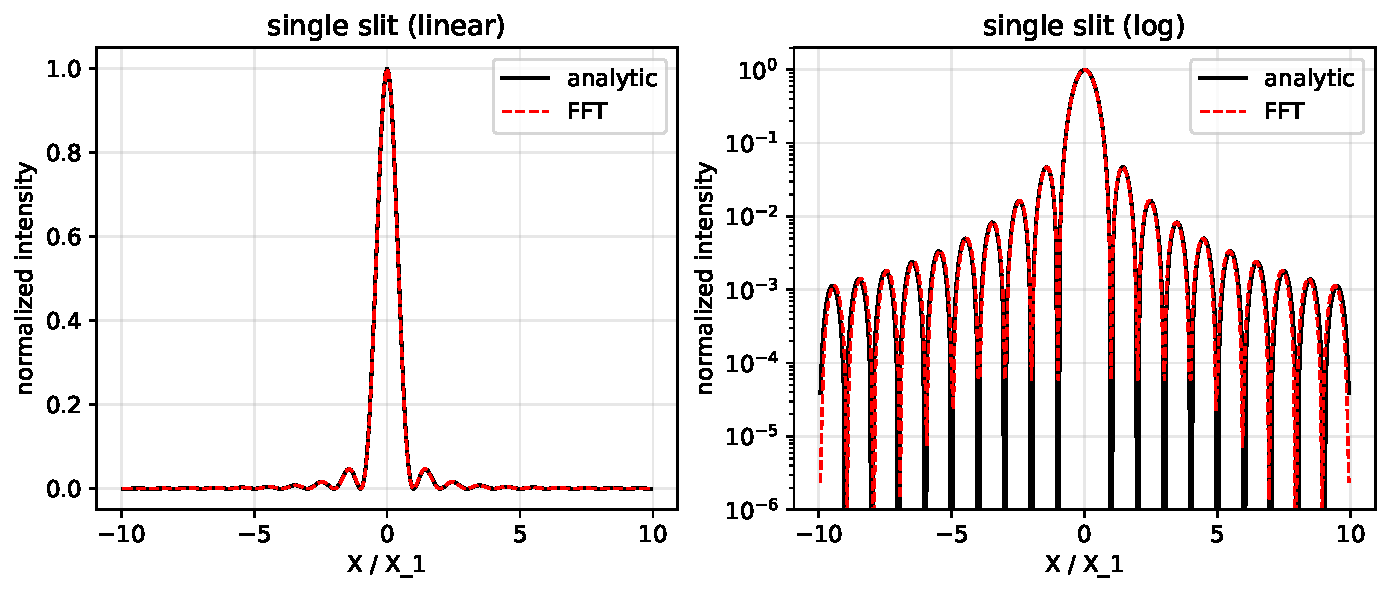
\includegraphics[width=0.47\textwidth]{../figures/experiment1_single_slit.pdf}
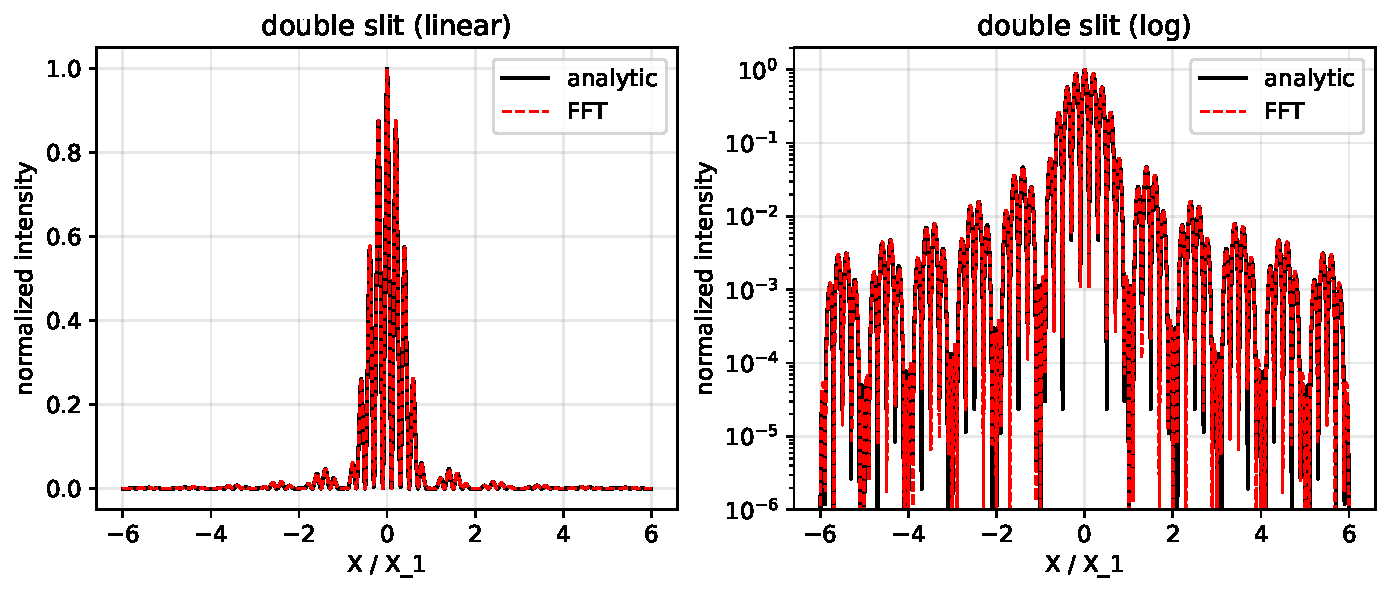
\includegraphics[width=0.47\textwidth]{../figures/experiment1_double_slit.pdf}\\[0.3em]
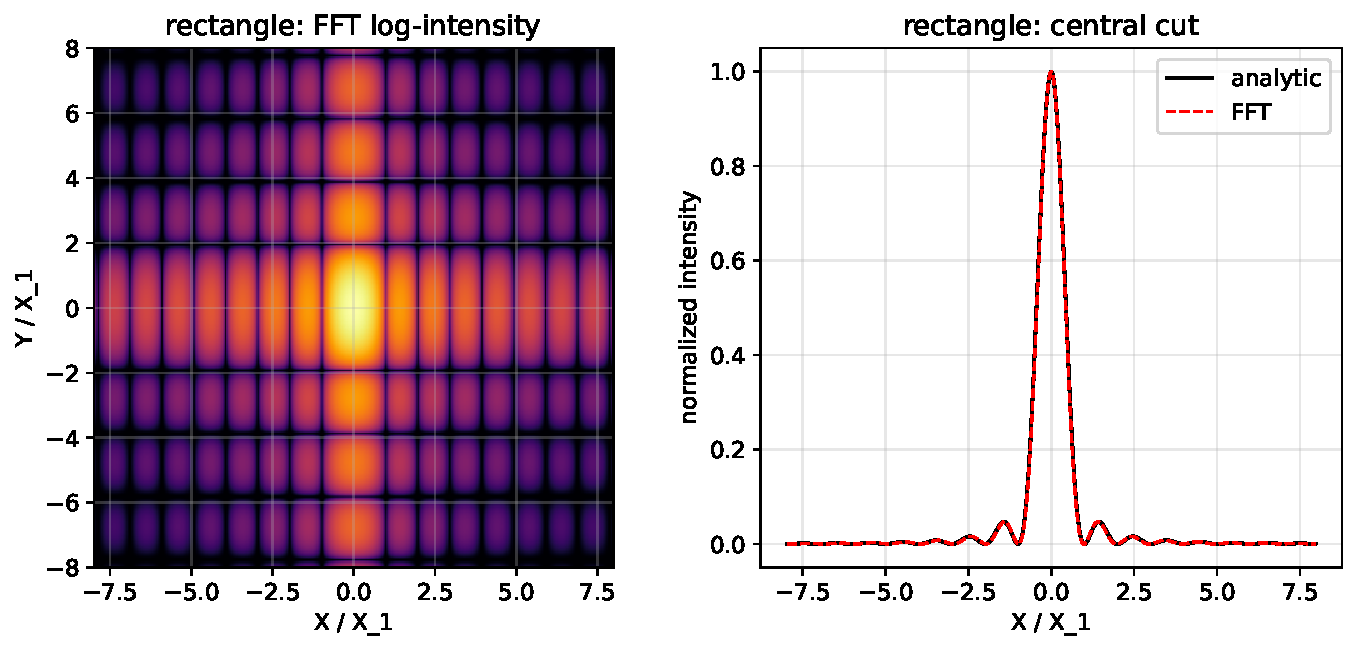
\includegraphics[width=0.47\textwidth]{../figures/experiment1_rectangle.pdf}
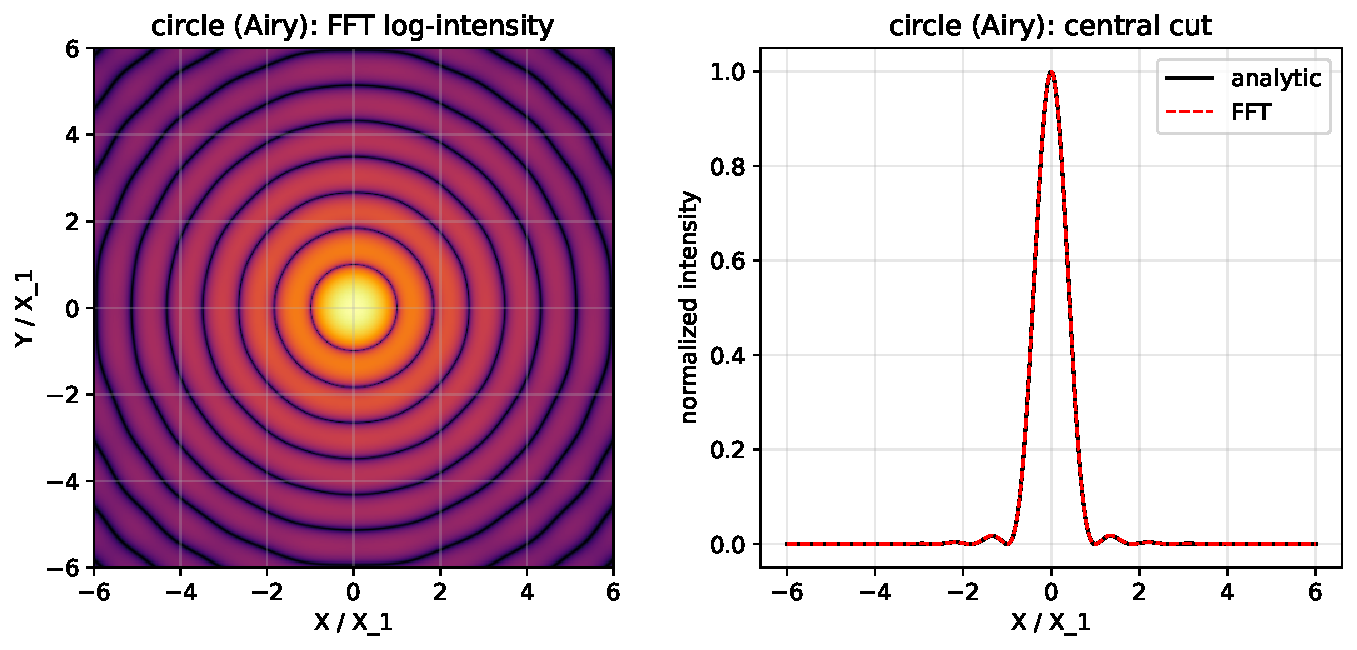
\includegraphics[width=0.47\textwidth]{../figures/experiment1_circle.pdf}
\caption{Experiment 1. Analytical validation for single slit, double slit, rectangular aperture, and
circular aperture.}
\label{fig:exp1}
\end{figure}

\subsection{Experiment 2: Convergence Rates}

The second experiment studies how the error decreases as the aperture sampling is refined. The physical
window is fixed at \(L=4\,\mathrm{mm}\), and \(N=2^k\) is varied from \(64\) to \(4096\). Thus
\(\Delta x=L/N\) decreases while the screen spacing \(\Delta X=\lambda z/L\) stays fixed. Two apertures
are compared: a square aperture with jump discontinuities and a Gaussian aperture with rapidly decaying
spectrum.

The square aperture has fitted slope \(-0.967\), very close to the expected \(O(1/N)\) behavior. The
Gaussian aperture reaches machine precision by \(N=256\). This confirms the central point from the error
analysis: the convergence rate is determined by the aperture's smoothness and spectral decay, not by the
FFT algorithm alone.

\begin{figure}[H]
\centering
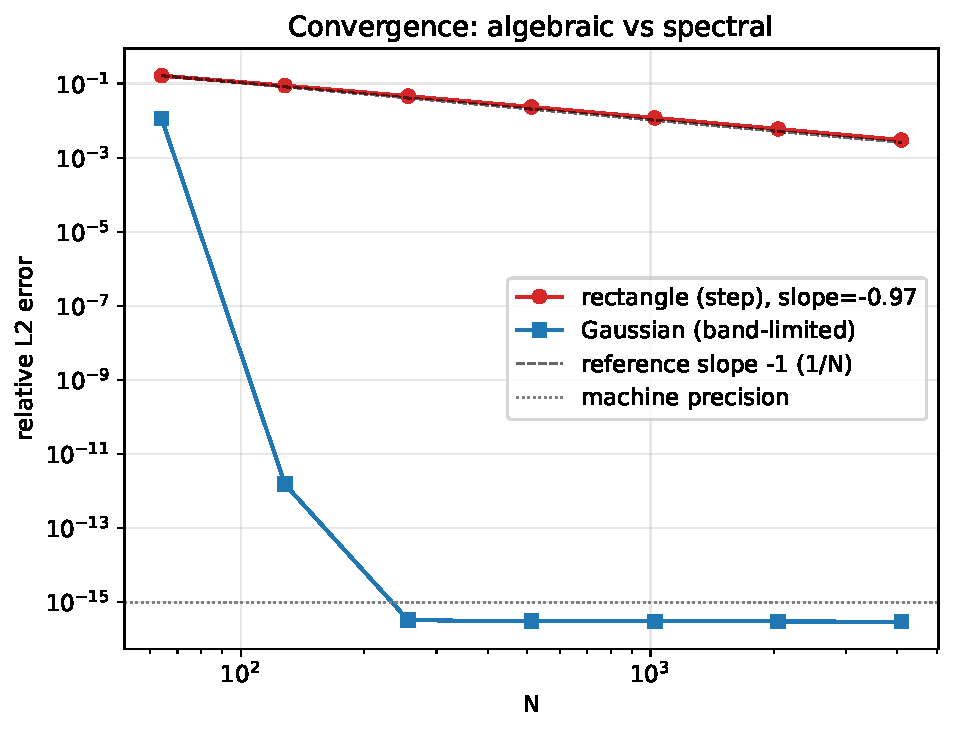
\includegraphics[width=0.62\textwidth]{../figures/experiment2_convergence.pdf}
\caption{Experiment 2. Relative \(L^2\) error versus \(N\). The discontinuous aperture follows an
approximately \(1/N\) trend, while the Gaussian aperture rapidly reaches machine precision.}
\label{fig:exp2}
\end{figure}

\subsection{Experiment 3: Validation of Grid Design Rules}

The third experiment tests whether the grid-design formulas in Section 4 give a tight lower bound. Two
scenarios isolate the two FFT grid constraints. In the first, \(L\) is fixed and \(\Delta x\) is varied to
test aliasing. In the second, \(\Delta x\) is fixed and \(L\) is varied to test screen resolution.

\begin{table}[H]
\centering
\small
\begin{tabular}{c|c|c}
Scale & E1 aliasing error & E2 resolution error \\
\hline
\(0.5\times\) & \(3.547\times10^{-2}\) & \(5.325\times10^{-2}\) \\
\(1\times\) design & \(1.398\times10^{-9}\) & \(1.392\times10^{-3}\) \\
\(2\times\) & \(3.788\times10^{-16}\) & \(4.086\times10^{-3}\)
\end{tabular}
\caption{Grid-design tightness test. The \(0.5\times\) grids fail, while the designed grids already meet
the target accuracy.}
\label{tab:exp3}
\end{table}

For E1, the half-size grid cuts into the Gaussian spectrum and produces a \(3.5\%\) error, while the
designed grid reduces the error to \(10^{-9}\). For E2, the half-size grid samples the double-slit fringes
too sparsely and gives a \(5.3\%\) error. Doubling beyond the designed grid gives almost no useful
improvement, which supports the claim that the design formulas are tight rather than excessively
conservative.

\begin{figure}[H]
\centering
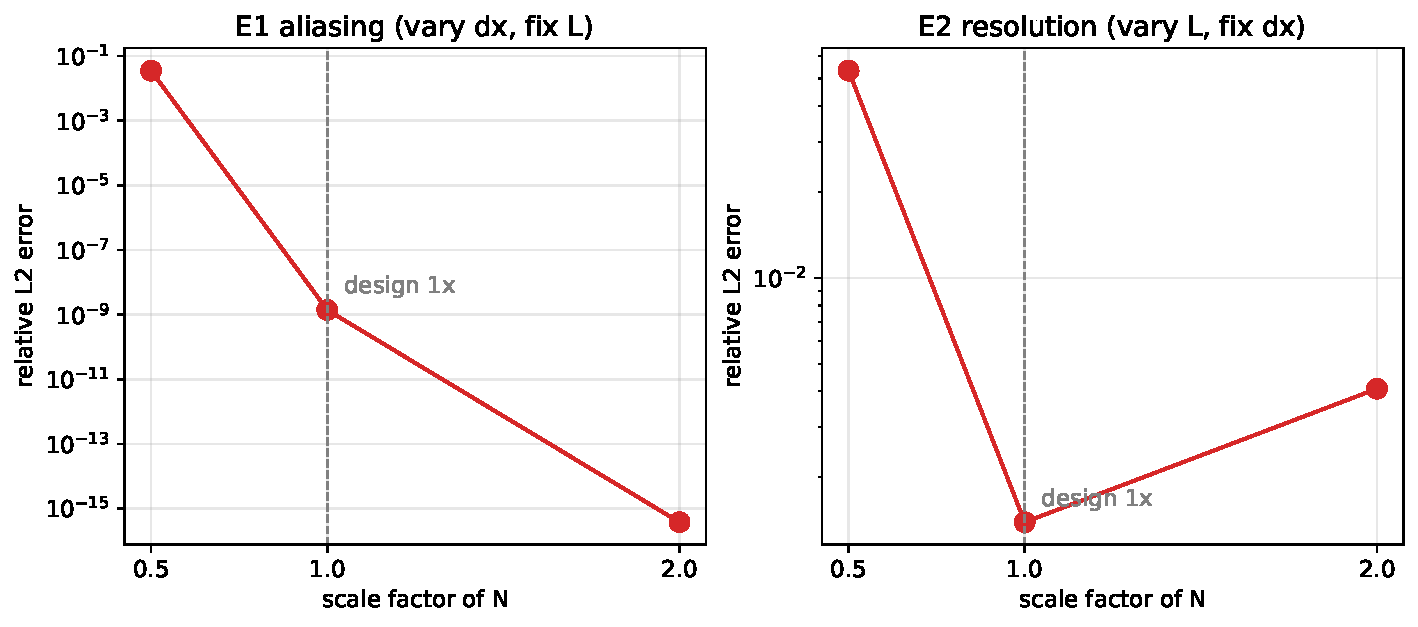
\includegraphics[width=0.48\textwidth]{../figures/experiment3_tightness.pdf}
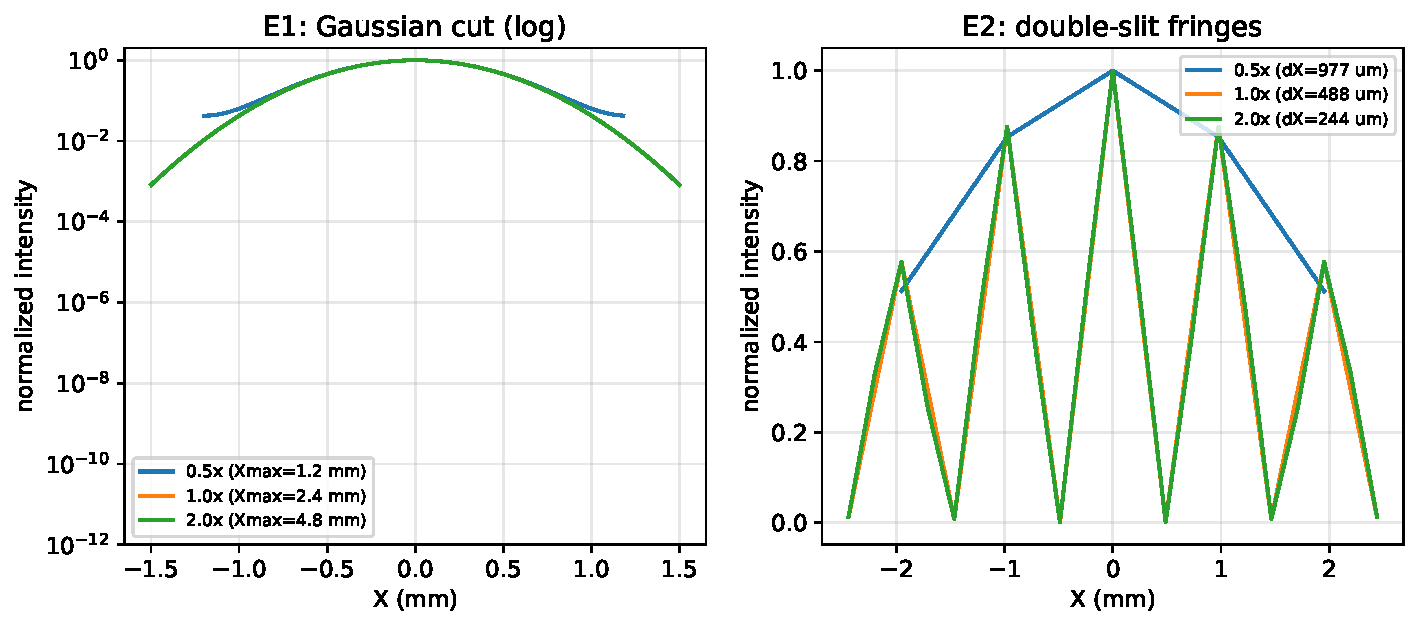
\includegraphics[width=0.48\textwidth]{../figures/experiment3_patterns.pdf}
\caption{Experiment 3. Left: error versus grid scale. Right: representative profiles showing aliasing
and screen under-resolution at the \(0.5\times\) grid.}
\label{fig:exp3}
\end{figure}

\subsection{Experiment 4: Breakdown of the Fraunhofer Approximation}

The fourth experiment isolates the model error E3. A circular aperture of radius \(a=0.2\,\mathrm{mm}\)
is propagated with \(\lambda=500\,\mathrm{nm}\), \(N=512\), and \(\Delta x=a/40\). The distance \(z\) is
chosen so that the Fresnel number \(F=a^2/(\lambda z)\) ranges from \(10^{-3}\) to \(10^1\). Fraunhofer is
compared with the single-FFT Fresnel propagator on the same screen grid, so the difference is precisely
the aperture-plane quadratic phase that Fraunhofer neglects.

\begin{table}[H]
\centering
\small
\begin{tabular}{c|c|c|c}
\(F\) & E3 & \(F\) & E3 \\
\hline
\(1.0\times10^{-3}\) & \(3.55\times10^{-7}\) & \(4.64\times10^{-1}\) & \(8.16\times10^{-2}\) \\
\(1.0\times10^{-2}\) & \(3.55\times10^{-5}\) & \(1.00\times10^{0}\) & \(4.54\times10^{-1}\) \\
\(1.0\times10^{-1}\) & \(3.56\times10^{-3}\) & \(2.15\times10^{0}\) & \(9.94\times10^{-1}\) \\
\(2.15\times10^{-1}\) & \(1.67\times10^{-2}\) & \(1.00\times10^{1}\) & \(1.00\times10^{0}\)
\end{tabular}
\caption{Fraunhofer model error as a function of the Fresnel number.}
\label{tab:exp4}
\end{table}

For small \(F\), the fitted slope is \(2.00\), consistent with \(\mathrm{E3}\sim F^2\). Around \(F=1\),
the error reaches about \(0.45\), and for \(F\gtrsim3\) it saturates near \(1\). An ASM cross-check at
\(F=3\) agrees with the Fresnel-FFT reference to relative \(L^2\) error \(5.4\times10^{-3}\), confirming
that the reference solution is reliable.

\begin{figure}[H]
\centering
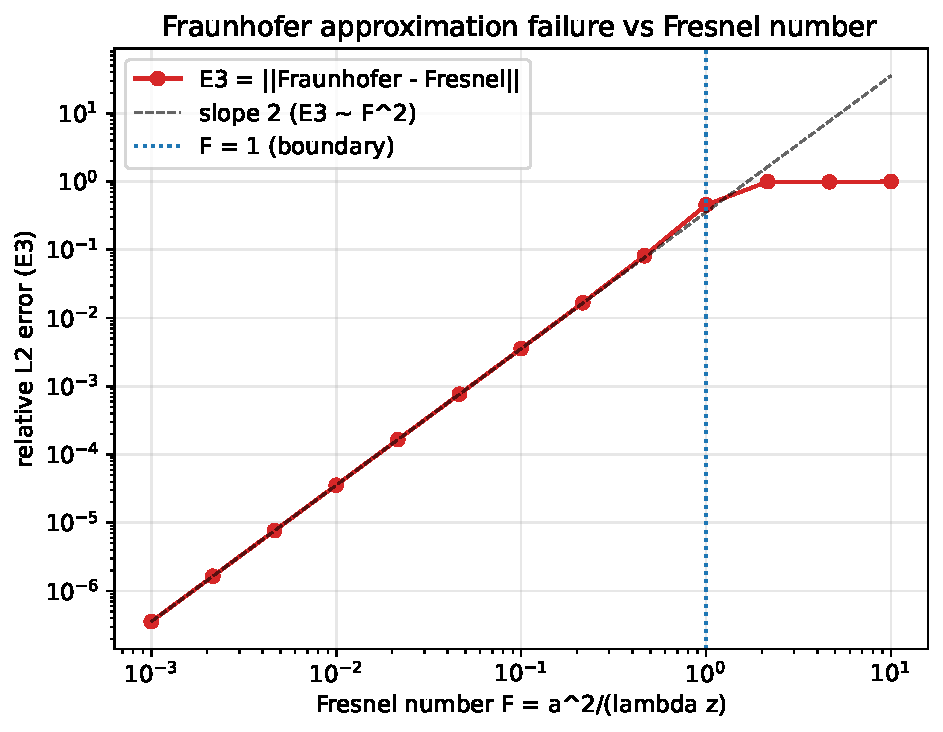
\includegraphics[width=0.48\textwidth]{../figures/experiment4_e3_vs_fresnel.pdf}
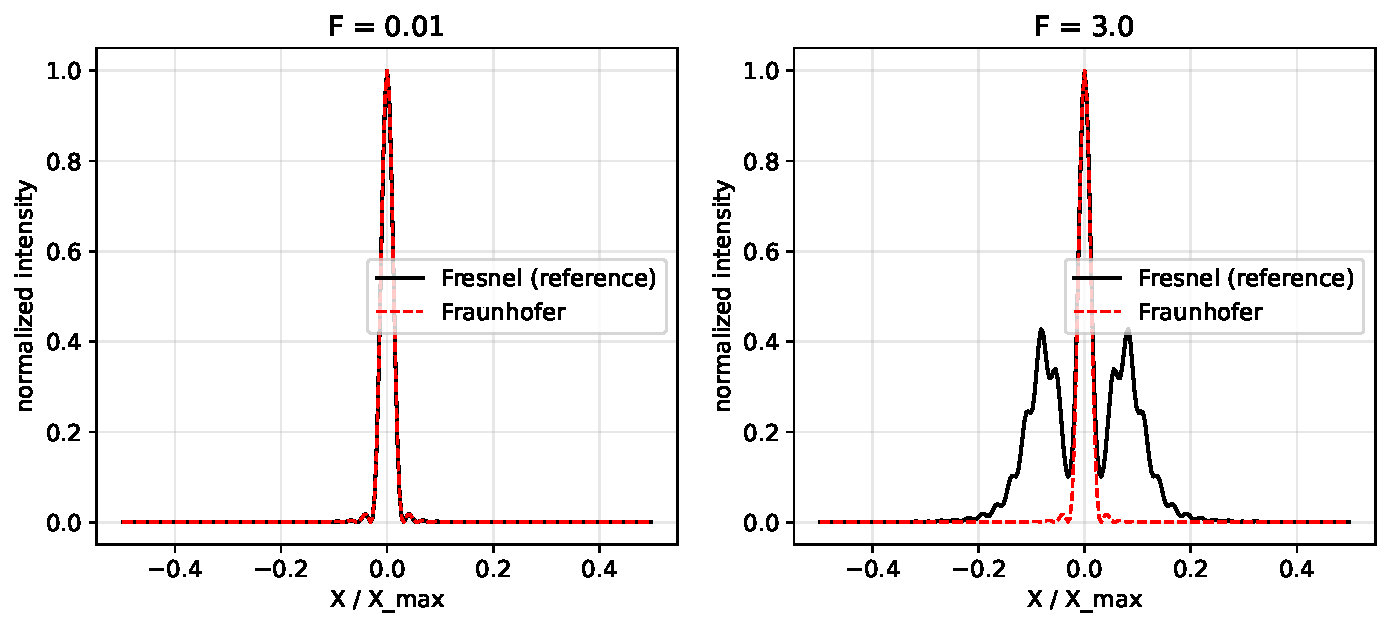
\includegraphics[width=0.48\textwidth]{../figures/experiment4_patterns.pdf}
\caption{Experiment 4. Left: E3 versus Fresnel number. Right: center profiles in a valid far-field case
and a near-field failure case.}
\label{fig:exp4}
\end{figure}

\subsection{Experiment 5: Efficiency Comparison}

The fifth experiment compares the FFT propagator with direct Simpson quadrature on a Gaussian aperture.
The Gaussian is used because both algorithms reach essentially the same accuracy in the central region, so
the timing comparison is not confounded by different error levels. The FFT computes a full \(N\times N\)
screen in \(O(N^2\log N)\), while direct Simpson quadrature on the same \(N\times N\) screen grid costs
\(O(N^4)\).

\begin{table}[H]
\centering
\small
\begin{tabular}{c|c|c|c}
\(N\) & FFT time (s) & Simpson time (s) & Speedup \\
\hline
64 & \(2.5\times10^{-4}\) & \(1.68\times10^{-1}\) & \(\sim670\times\) \\
128 & \(9.6\times10^{-4}\) & \(2.09\times10^{0}\) & \(\sim2200\times\) \\
256 & \(9.4\times10^{-3}\) & \(6.16\times10^{1}\) & \(\sim6500\times\) \\
512 & \(5.97\times10^{-2}\) & -- & -- \\
4096 & \(6\)--\(10\) & -- & --
\end{tabular}
\caption{Timing comparison between FFT propagation and direct Simpson quadrature.}
\label{tab:exp5}
\end{table}

The fitted FFT slope is \(2.43\), consistent with \(O(N^2\log N)\), while the Simpson slope is \(3.87\),
consistent with \(O(N^4)\). At \(N=256\), the FFT is already about \(6500\) times faster. The measured
relative \(L^2\) differences between FFT and Simpson at \(N=64\) and \(N=128\) are \(5.9\times10^{-15}\)
and \(3.4\times10^{-16}\), respectively, confirming that the timing comparison is made at the same
accuracy level.

\subsection{Experiment 6: Rayleigh Criterion Recovery}

The sixth experiment is the main physical target of the project. A circular aperture of diameter \(D\) is
sampled with \(\Delta x=D/128\), its Airy pattern is computed by the FFT propagator, and the first dark
ring radius \(r_1\) is located from the central horizontal cut using a three-point parabolic refinement.
The recovered dimensionless constant is \(c_{\mathrm{num}}=r_1D/(\lambda z)\), to be compared with
\(1.2196699\ldots\).

\begin{table}[H]
\centering
\small
\begin{tabular}{c|c|c|c}
\(N\) & Samples per first ring & \(c_{\mathrm{num}}\) & Relative error \\
\hline
512 & 4.9 & 1.299592 & \(6.55\times10^{-2}\) \\
1024 & 9.8 & 1.238582 & \(1.55\times10^{-2}\) \\
2048 & 19.5 & 1.221345 & \(1.37\times10^{-3}\) \\
4096 & 39.1 & 1.220777 & \(9.08\times10^{-4}\) \\
8192 & 78.1 & 1.219887 & \(1.78\times10^{-4}\)
\end{tabular}
\caption{Numerical recovery of the Rayleigh constant for \(D=0.5\,\mathrm{mm}\).}
\label{tab:exp6}
\end{table}

At \(N=8192\), the recovered value is \(c_{\mathrm{num}}=1.21989\), compared with
\(c_{\mathrm{exact}}=1.21967\), giving a relative error of \(1.78\times10^{-4}\), or \(0.018\%\). At
fixed \(N=4096\), changing \(D/\lambda\) over \(500,1000,2000,4000\) gives the same recovered value
\(1.220777\), confirming the expected scale invariance of the Fraunhofer Airy pattern.

\begin{figure}[H]
\centering
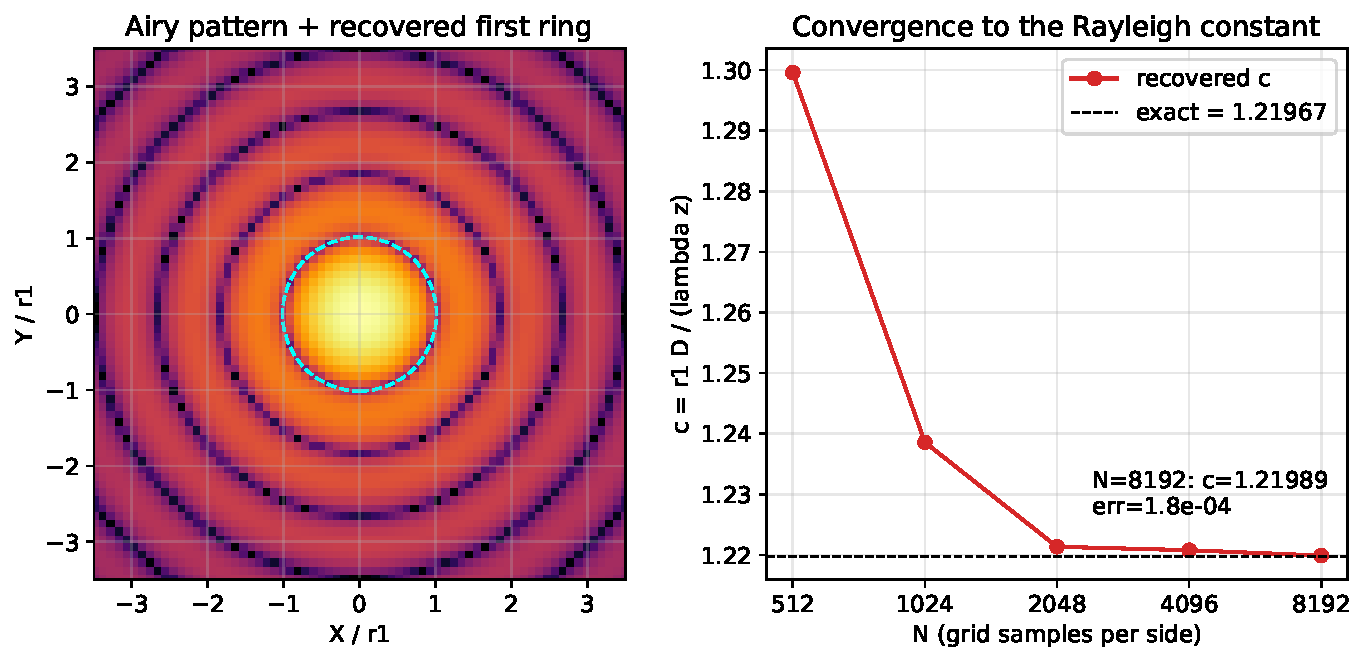
\includegraphics[width=0.82\textwidth]{../figures/experiment6_rayleigh.pdf}
\caption{Experiment 6. Airy pattern with the recovered first dark ring, and convergence of the recovered
Rayleigh constant.}
\label{fig:exp6}
\end{figure}

\subsection{Experiment 7: Complex Apertures}

The final experiment applies the same FFT propagator to more complex apertures. These examples are mainly
demonstrations rather than error studies, but they show that the method handles nontrivial aperture
geometries without changing the algorithm.

\begin{figure}[H]
\centering
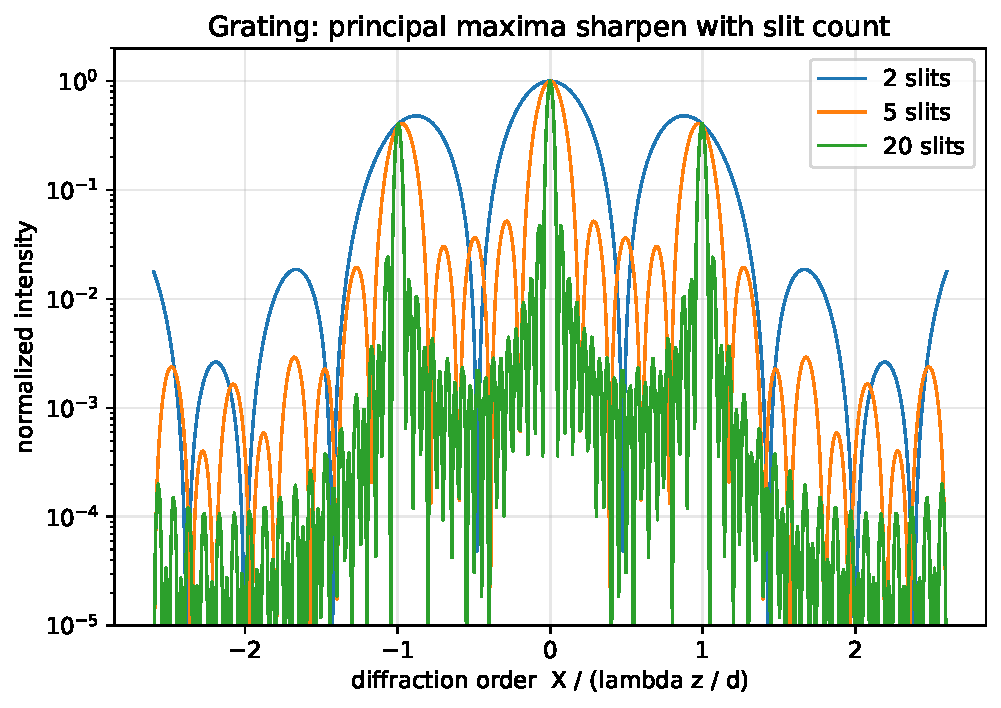
\includegraphics[width=0.48\textwidth]{../figures/experiment7_grating_slitcount.pdf}
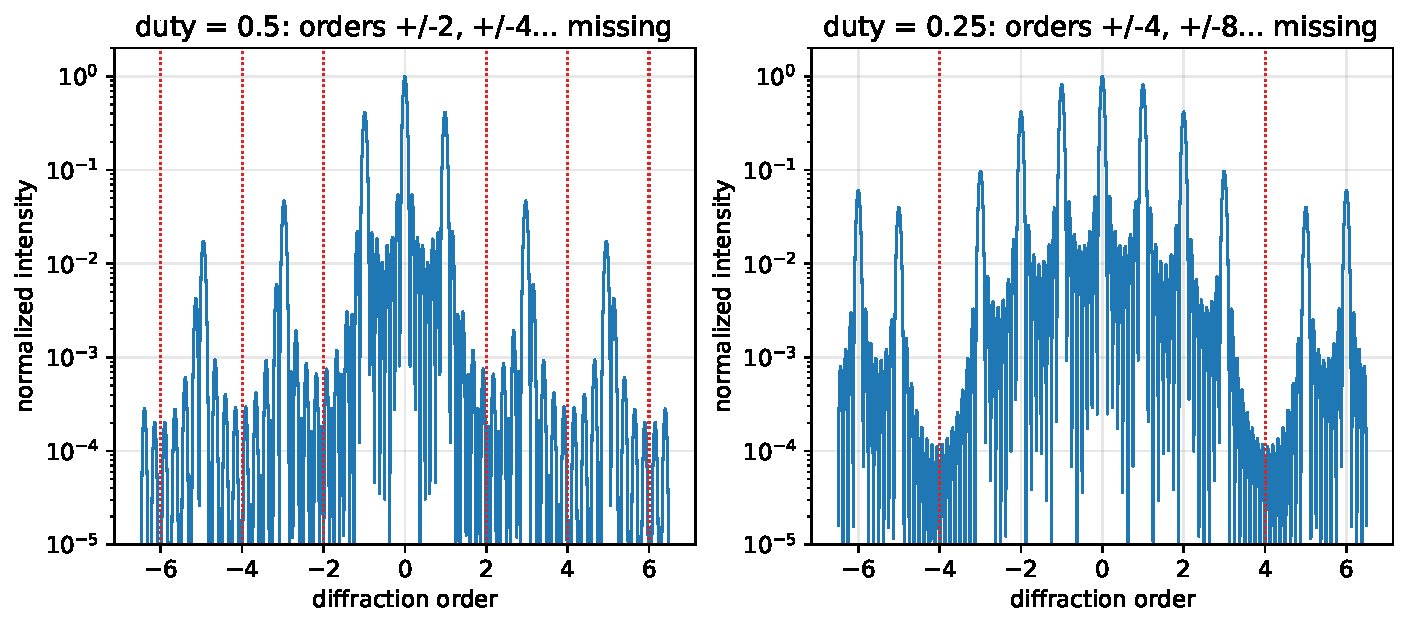
\includegraphics[width=0.48\textwidth]{../figures/experiment7_grating_duty.pdf}
\caption{Experiment 7, gratings. Left: increasing the number of slits sharpens the principal maxima.
Right: changing the duty cycle creates missing diffraction orders.}
\label{fig:exp7_grating}
\end{figure}

For the grating examples, the principal maxima occur at integer diffraction orders. Increasing the slit
number from \(2\) to \(20\) narrows the peaks and increases the resolving power. Changing the duty cycle
produces missing orders: duty cycle \(0.5\) suppresses the even orders, while duty cycle \(0.25\) suppresses
orders that are multiples of \(4\).

\begin{figure}[H]
\centering
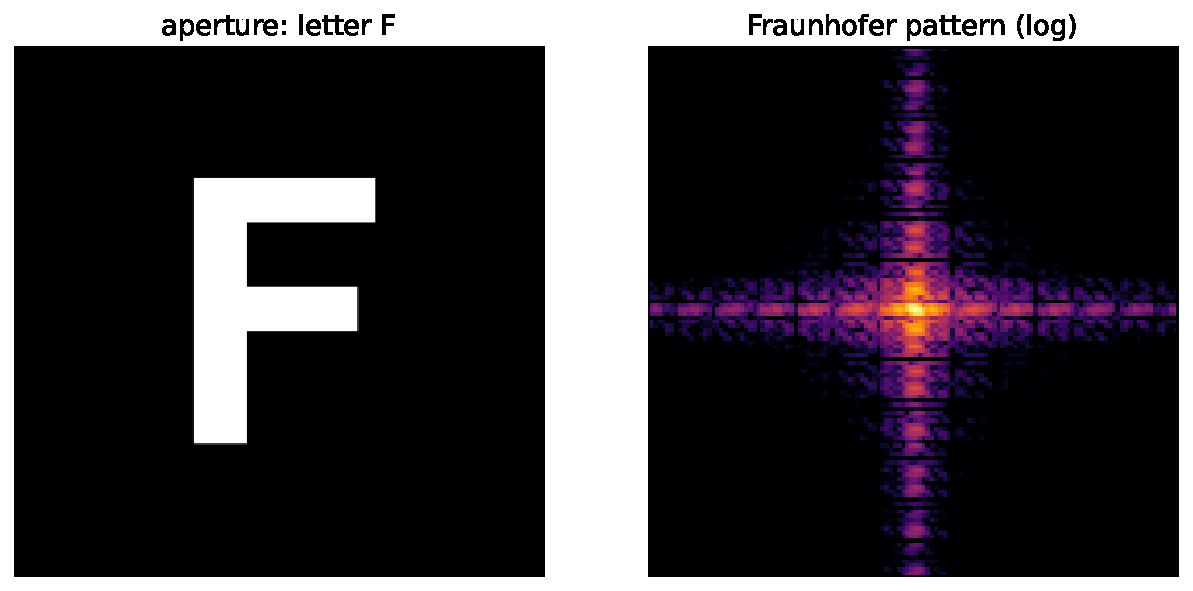
\includegraphics[width=0.48\textwidth]{../figures/experiment7_letter.pdf}
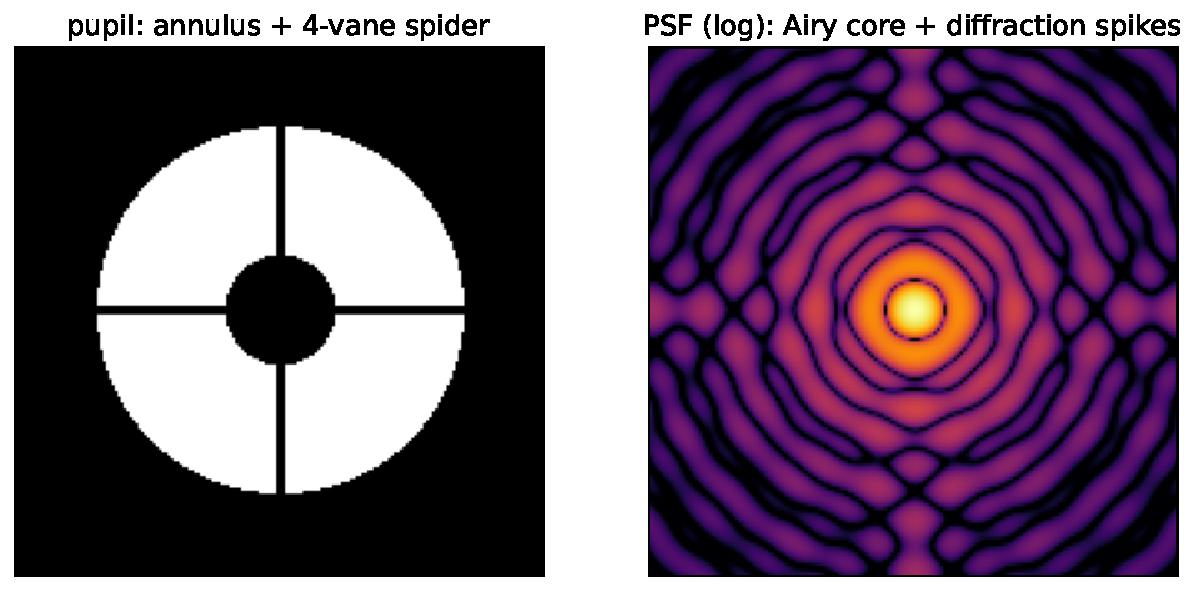
\includegraphics[width=0.48\textwidth]{../figures/experiment7_telescope.pdf}
\caption{Experiment 7, complex pupils. Left: a letter-shaped aperture. Right: an annular telescope pupil
with support struts and its PSF.}
\label{fig:exp7_complex}
\end{figure}

The letter aperture produces strong horizontal and vertical spectral structures associated with its
straight edges. The telescope pupil produces an Airy-like core modified by the central obstruction, along
with diffraction spikes caused by the support struts. These qualitative results agree with the Fourier
interpretation of aperture geometry and far-field intensity.

\section{Conclusion}

This project derived the Fraunhofer diffraction formula from the angular-spectrum and Fresnel viewpoints,
then implemented it as an FFT-based numerical method. The derivation also fixed the grid interpretation:
the aperture spacing \(\Delta x\) determines the non-aliased screen range, while the window length
\(L=N\Delta x\) determines the screen spacing \(\Delta X=\lambda z/L\).

The experiments validate this sampling picture. Analytical apertures agree with their closed-form
patterns, discontinuous and smooth apertures show the expected difference in convergence behavior, and the
grid-design tests confirm that \(\Delta x\), \(L\), and the Fresnel number \(F=a^2/(\lambda z)\) control
different errors. The efficiency comparison also shows why the FFT is the practical algorithm for
two-dimensional diffraction: it reproduces direct quadrature in the tested regime while reducing the cost
from \(O(N^4)\) to \(O(N^2\log N)\).

Finally, the Rayleigh-criterion experiment connects the computation to a concrete optical prediction. The
recovered Airy-disk constant converges to \(1.21967\ldots\), giving a direct numerical verification of the
classical resolution scale \(1.22\lambda/D\). The resulting report is therefore a self-contained numerical
realization of standard Fourier-optics theory \cite{goodman2017,mit271} and its FFT implementation practice
\cite{douglass}.

\section*{Acknowledgement}
\addcontentsline{toc}{section}{Acknowledgement}

I would like to thank ChatGPT for helping me learn the optical background needed for this project and for
assisting with the polishing of this report. Its explanations were useful in connecting the Fourier-optics
theory with the numerical implementation, while all final choices, computations, and responsibility for the
report remain my own.

\phantomsection
\addcontentsline{toc}{section}{References}
\begin{thebibliography}{9}

\bibitem{goodman2017}
J. W. Goodman, \textit{Introduction to Fourier Optics}, 4th ed., W. H. Freeman, 2017.

\bibitem{mit271}
MIT OpenCourseWare, \textit{2.71 Optics}, Lectures 15--17.

\bibitem{douglass}
K. M. Douglass, ``Approximating Diffraction Patterns of Rectangular Apertures with the FFT,''
\url{https://kmdouglass.github.io/posts/approximating-diffraction-patterns-of-rectangular-apertures-with-the-fft/}.

\end{thebibliography}

\end{document}
